\documentclass[
  a4paper,
  12pt,
  english,
  brazilian,
]{article}

%% Pacotes utilizados
\usepackage[]{fatec-article}
\usepackage{float} % Para usar o modificador H

%% Início do documento
\begin{document}
\vspace{8cm}
\begin{center}
    \large \textbf{\title{ARTEFATOS DO PROJETO CALM WAVE}}
\end{center}

\maketitle

\break

\tableofcontents

\break

\section*{Artefatos do Projeto}
Esta seção apresenta os artefatos utilizados para modelar e desenvolver o sistema Calm Wave, um dispositivo antirruído adaptativo com inteligência artificial para auxiliar indivíduos com TPAC.

\subsection*{Canvas do Projeto}
\addcontentsline{toc}{section}{Canvas do Projeto}

O Canvas do projeto apresenta uma visão geral da proposta de valor e modelo de negócio do Calm Wave, sendo o primeiro passo para entender o escopo e objetivos do projeto.

\begin{figure}[H]
\centering
\caption{Canvas do projeto Calm Wave}%
\label{fig:canvas-projeto}
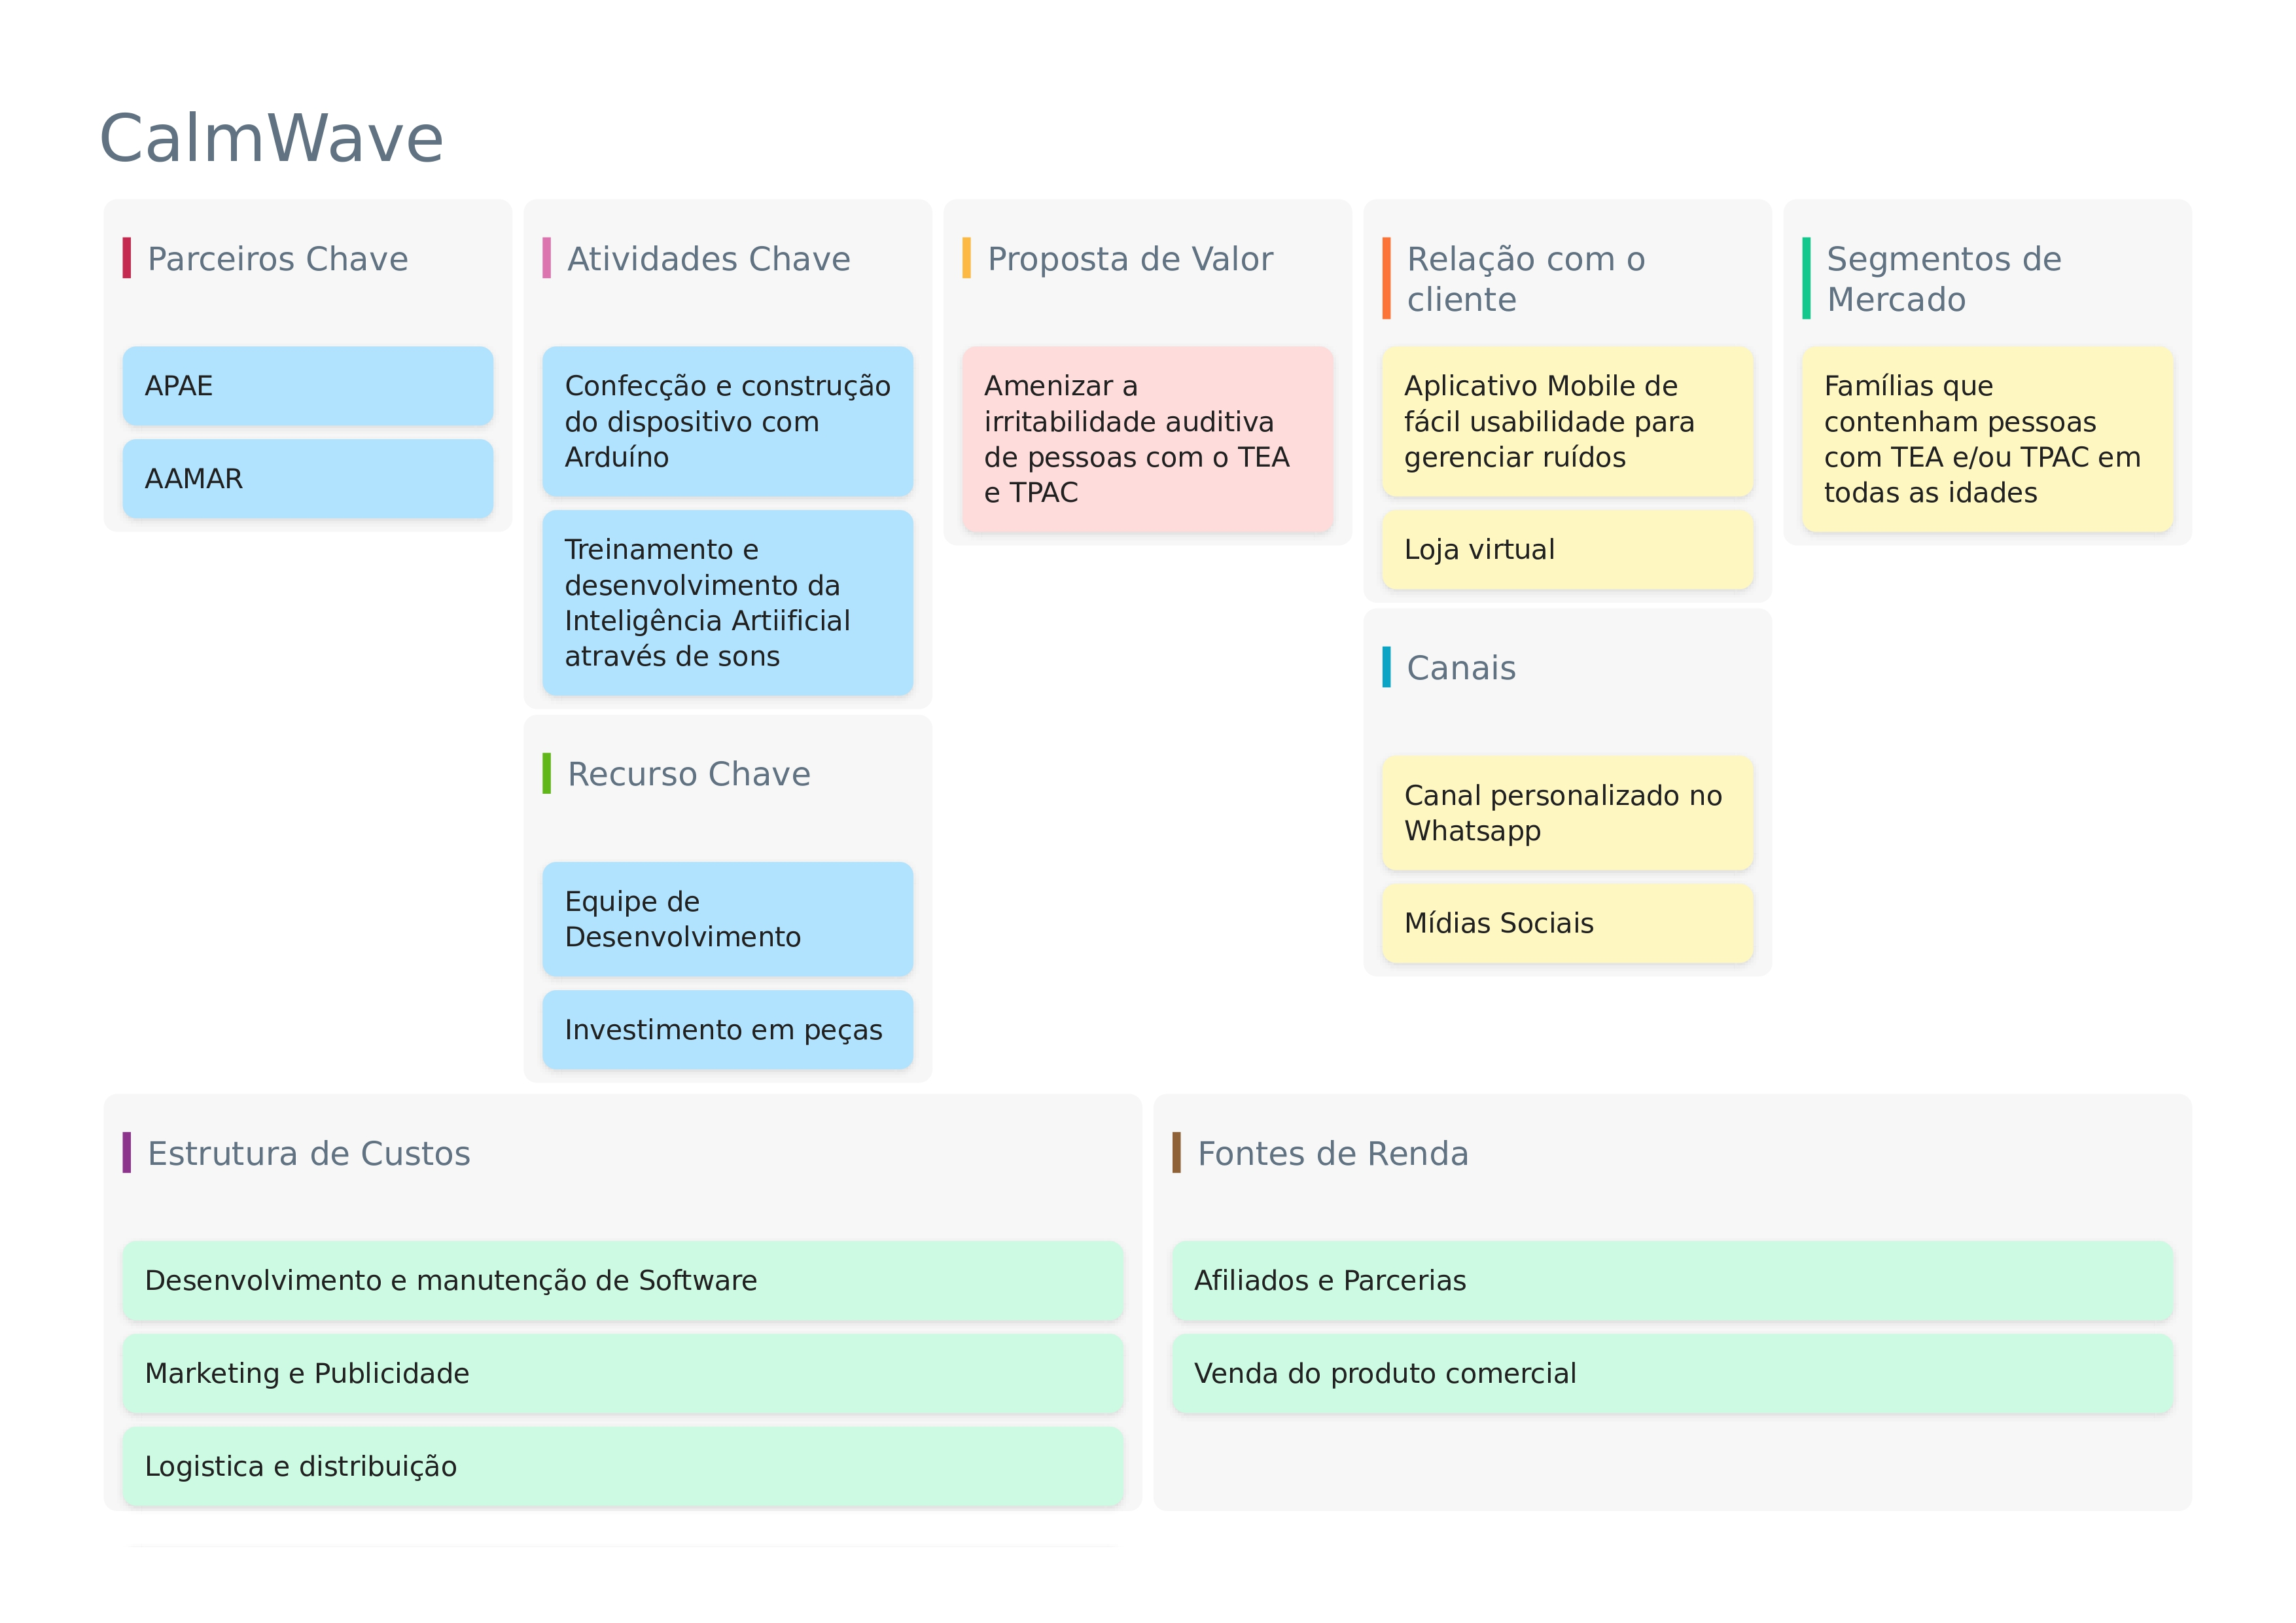
\includegraphics[width=0.8\textwidth]{Logos/Canva_calm_wave.jpg}
\SourceOrNote{Autores (2024)}
\end{figure}

Este Canvas demonstra os principais aspectos do projeto, incluindo proposta de valor, segmentos de clientes e recursos necessários.

\subsection*{Diagrama de Caso de Uso}
\addcontentsline{toc}{section}{Diagrama de Caso de Uso}

Após definir o modelo de negócio, o diagrama de caso de uso representa as principais interações entre os diferentes tipos de usuários e o sistema Calm Wave, demonstrando as funcionalidades básicas que precisam ser implementadas.

\begin{figure}[H]
\centering
\caption{Diagrama de caso de uso do Calm Wave}%
\label{fig:diagrama-caso-uso}
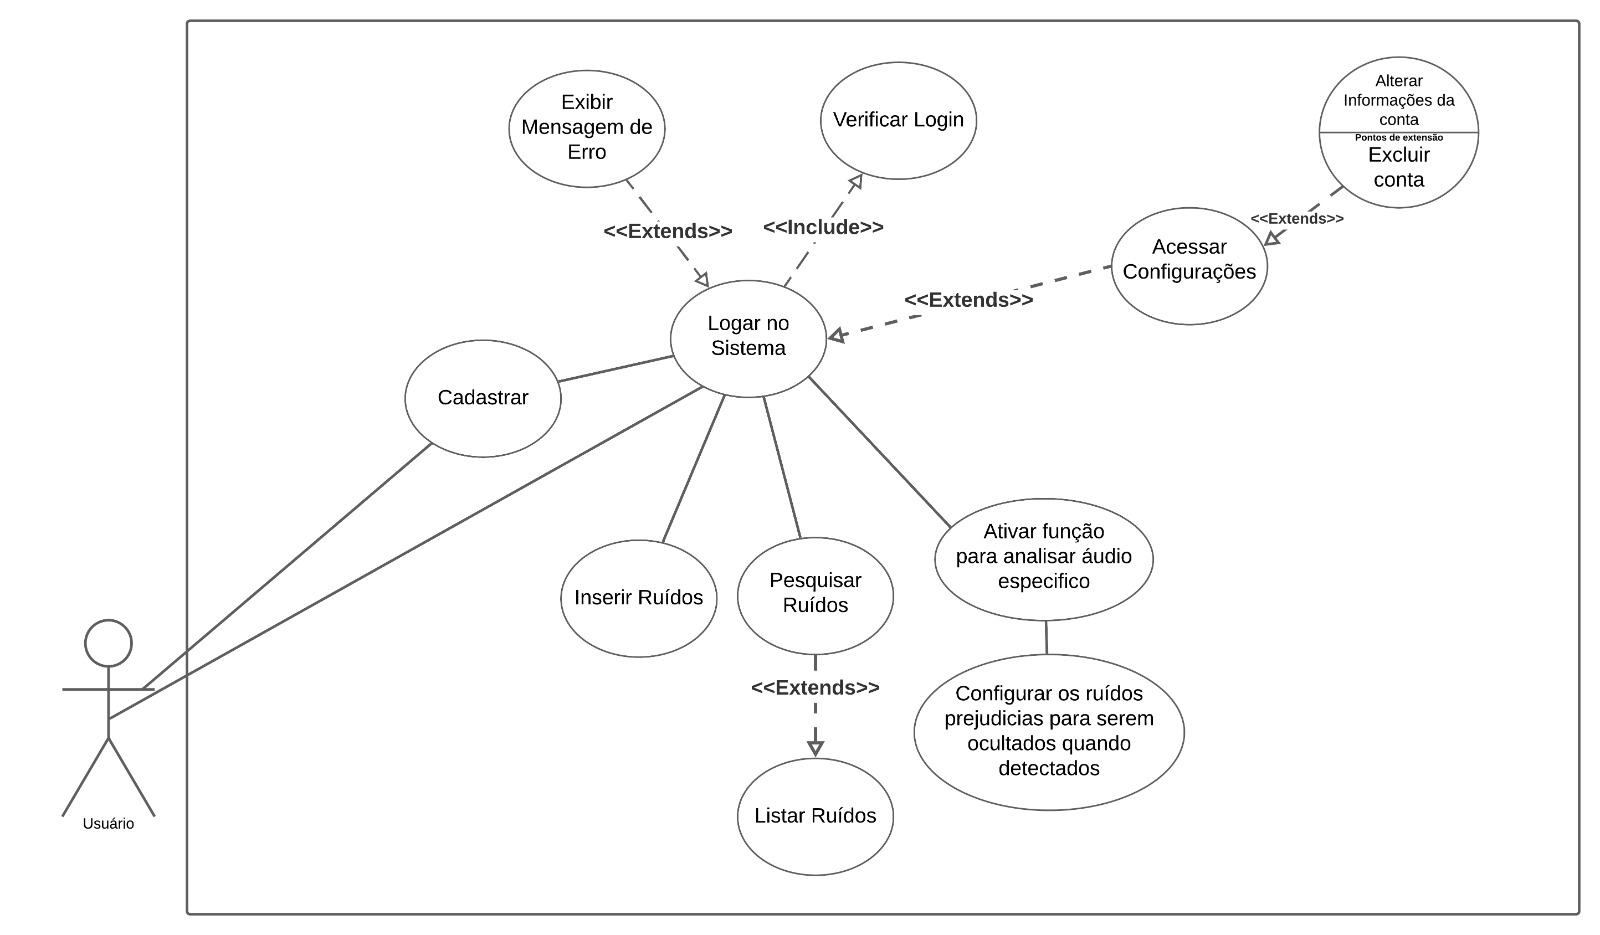
\includegraphics[width=1.1\textwidth]{Logos/Caso_de_uso.jpg}
\SourceOrNote{Autores (2024)}
\end{figure}

O diagrama ilustra como o sistema interage com seus usuários para proporcionar suas funcionalidades principais.

\subsection*{Diagrama de Classe}
\addcontentsline{toc}{section}{Diagrama de Classe}

Com base nas funcionalidades identificadas, o diagrama de classe representa a estrutura do sistema, mostrando as principais classes e seus relacionamentos necessários para implementação.

\begin{figure}[H]
\centering
\caption{Diagrama de classe do Calm Wave}%
\label{fig:diagrama-classe}
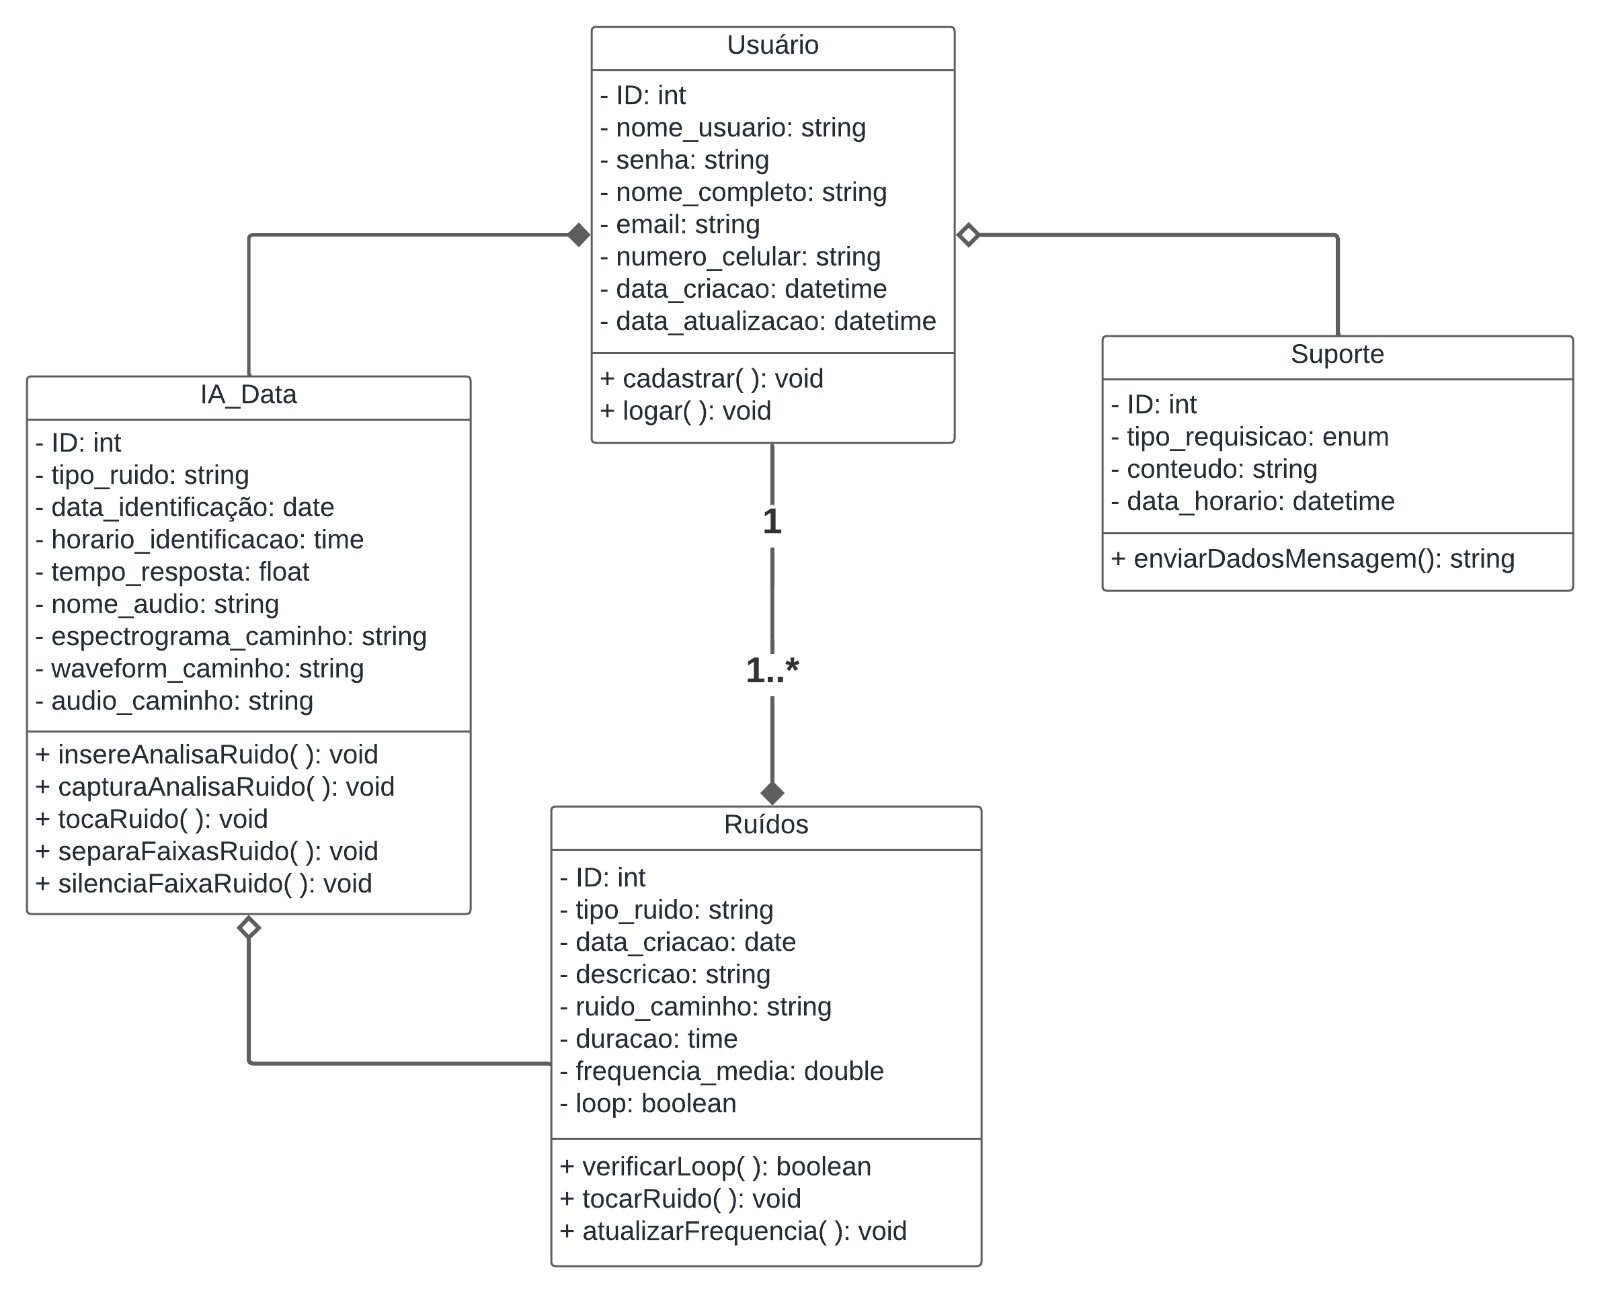
\includegraphics[width=0.8\textwidth]{Logos/Diagrama_classes.jpg}
\SourceOrNote{Autores (2024)}
\end{figure}

Esta estrutura demonstra a organização dos componentes do sistema.

\subsection*{Diagrama de Objetos}
\addcontentsline{toc}{section}{Diagrama de Objetos}

Para melhor compreensão da implementação, o diagrama de objetos apresenta uma instância específica do sistema em funcionamento.

\begin{figure}[H]
\centering
\caption{Diagrama de objetos do Calm Wave}%
\label{fig:diagrama-objetos}
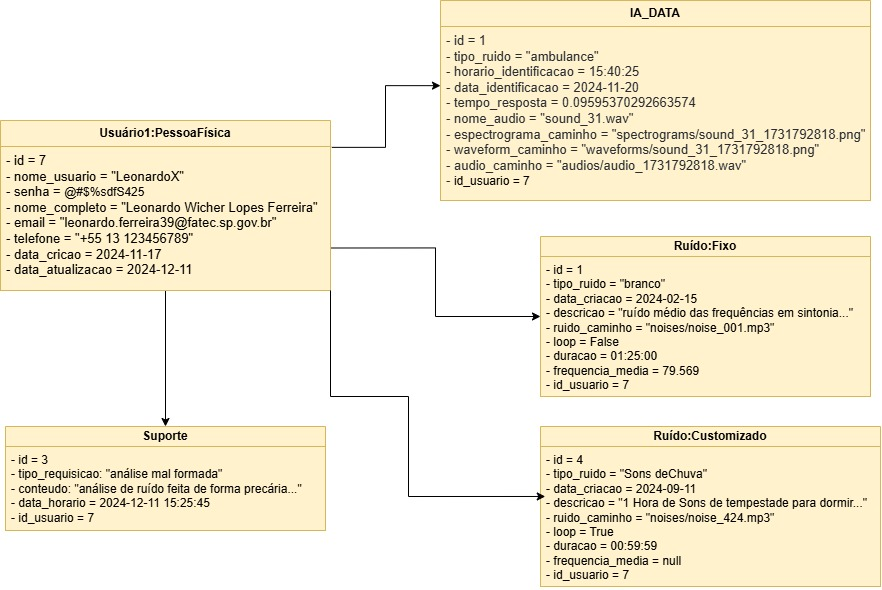
\includegraphics[width=0.8\textwidth]{Logos/Diagrama_objetos.jpg}
\SourceOrNote{Autores (2024)}
\end{figure}

Este diagrama ilustra um cenário de uso do sistema, mostrando como os diferentes componentes interagem entre si.

\subsection*{Modelo Lógico do Banco de Dados}
\addcontentsline{toc}{section}{Modelo Lógico do Banco de Dados}

Por fim, o modelo lógico apresenta a estrutura do banco de dados necessária para persistir as informações do sistema Calm Wave.

\begin{figure}[H]
\centering
\caption{Modelo lógico do banco de dados do Calm Wave}%
\label{fig:modelo-logico}
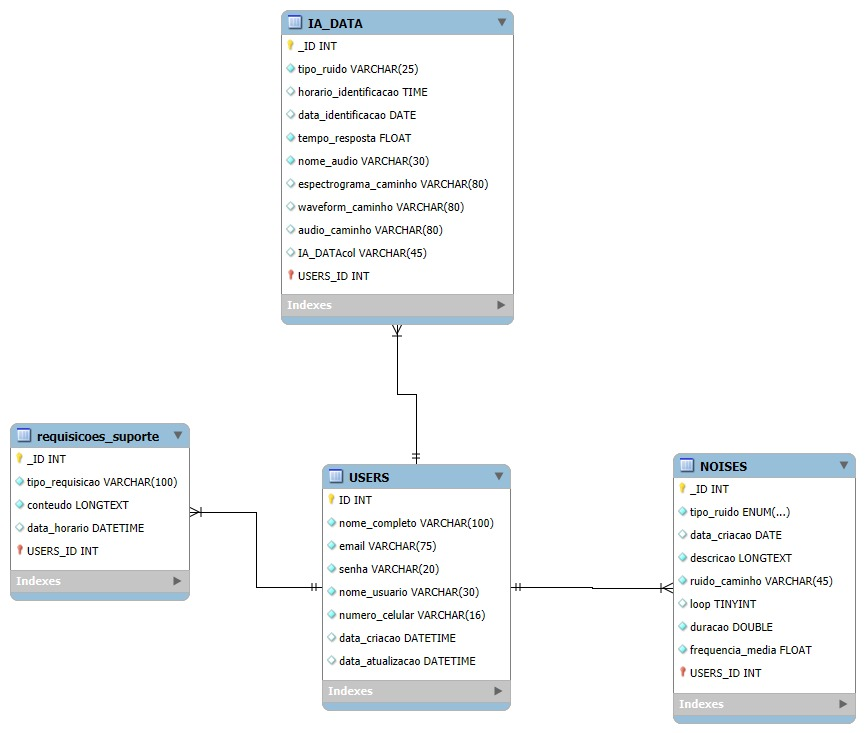
\includegraphics[width=0.8\textwidth]{Logos/Modelo_logico_banco.jpg}
\SourceOrNote{Autores (2024)}
\end{figure}

Este modelo representa a organização das tabelas e seus relacionamentos no banco de dados do sistema.

\end{document}
